\documentclass{article}

% NeurIPS-derived single-column preprint style. arxiv.sty ships alongside this
% file because it is not in a stock TeX Live tree. It loads geometry and fancyhdr
% itself, so neither is requested here; newtx is loaded after it so the Times it selects is the
% modern one with matching math rather than the base ptm.
\usepackage{arxiv}

\usepackage[utf8]{inputenc}
\usepackage[T1]{fontenc}
\usepackage{newtxtext,newtxmath}
\usepackage{microtype}
\usepackage{graphicx}
\usepackage{booktabs}
\usepackage{array}
\usepackage{multirow}
\usepackage{amsmath}
\usepackage{xcolor}
\usepackage[numbers,sort&compress]{natbib}
\usepackage{tikz}
\usetikzlibrary{arrows.meta,positioning,shapes.geometric,fit,backgrounds,calc}
\usepackage{pgfplots}
\pgfplotsset{compat=1.17}
\usepackage{algorithm}
\usepackage{algpseudocode}
\usepackage[colorlinks=true,linkcolor=blue!60!black,citecolor=blue!60!black,urlcolor=blue!60!black]{hyperref}
\usepackage[capitalise]{cleveref}
\usepackage{caption}
\captionsetup{font=small,labelfont=bf}

\definecolor{adblue}{HTML}{1F6FEB}
\definecolor{adgreen}{HTML}{3FB950}
\definecolor{adorange}{HTML}{D29922}
\definecolor{adred}{HTML}{CF222E}
\definecolor{adgray}{HTML}{57606A}

\newcommand{\evolve}{\texttt{evolve()}}
\newcommand{\code}[1]{\texttt{#1}}
\newcommand{\plugtitle}[1]{\textbf{\footnotesize #1}}
\newcommand{\Dval}{D_{\mathrm{val}}}

\title{AgentDescent: Asynchronous Parallel Self-Evolution of LLM Agents by Merging Conflicting Edits}

% Running head and the line under the title bar; the full title is too long to
% sit in a page header.
\renewcommand{\shorttitle}{AgentDescent}
\renewcommand{\undertitle}{}
\renewcommand{\headeright}{}

\author{
  Danyang Chen\\[2pt]
  \small\url{https://github.com/Birfy/agentdescent}
}

\date{August 2026}

\begin{document}
\maketitle

\begin{abstract}
A self-evolving agent loop pays for two things: rollouts, and the held-out validation that decides which proposed edit to keep. On live models the second dominates the critical path, and it is the one parallelism alone cannot reduce --- $N$ concurrent proposals mean $N$ acceptance tests. Merging removes that multiplier by validating a round's proposals once, but only where they can be fused, and they cannot when the artifact is held in a single key: every concurrent pair then conflicts, and merge-of-$N$ degenerates into best-of-$N$ selection at best-of-$N$ validation cost.

The fix is to merge the conflicting edits instead of discarding all but one: a model is asked to write their union --- one edit preserving what each proposal contributed --- and that union faces the same acceptance test as any candidate, so the model proposes and the gate decides. We call this \emph{reflective merge}. On an artifact where nothing else can fuse, the keyed union produces a fused candidate in $0$ of $48$ merges and reflective merge in $42$. That degeneracy is exact rather than rare, and it is the result we are most confident in. The same configuration also spends $40\%$ fewer model calls than the engine's shipped defaults at a pinned rollout budget (95\% CI $27$--$54\%$, same direction on every seed); we trace that saving to resolving conflicts by recombination rather than by ranking --- not, as we first assumed, to collapsing acceptance tests, since every configuration runs exactly one per merge. Quality is not the claim; at four seeds on a 30-task split we report the interval and do not assert equivalence. We also give a closed-form upper bound on how often merging can fire at all, which retrodicts two null results of our own. The framework these run on, \textbf{AgentDescent}, executes eighteen published self-evolution algorithms as plug-ins under serial, synchronous, and barrier-free schedulers without modification; on one of them, parallel execution reaches a median $6.8\times$ less wall-clock than a faithful serial control (three seeds, $3.1$--$9.5\times$). Code, workloads, and per-result reproduction commands are open source.
\end{abstract}

\keywords{Recursive self-improvement \and Self-evolving agents \and Parallel and asynchronous execution \and Diff aggregation \and Bounded staleness}

\section{Introduction}
\label{sec:intro}

A growing body of work shows that large-language-model agents can improve their own artifacts: prompts \citep{fernando2023promptbreeder,agrawal2025gepa}, in-context playbooks \citep{zhang2025ace}, skill libraries \citep{wang2023voyager,zheng2025skillweaver}, agentic workflows \citep{zhang2024aflow,hu2024adas}, and their own code \citep{zhang2025dgm,robeyns2025sica,yin2024godel}. Most of these systems share an execution structure inherited from the G\"odel machine \citep{schmidhuber2003godel}: a serial improvement loop in which one candidate modification is proposed, evaluated, and accepted or rejected before the next is considered. If one iteration takes $T_{\mathrm{iter}}$ wall-clock seconds, improvement throughput is bounded at one accepted change per $T_{\mathrm{iter}}$, independent of available compute. Notable exceptions parallelize at the \emph{population} level --- FunSearch and AlphaEvolve run asynchronous samplers over island archives \citep{romera2024funsearch,novikov2025alphaevolve} --- but their candidates remain independent: concurrent work is selected among, not merged.

Distributed deep learning encountered the same bottleneck and resolved it with a now-standard stack: data-parallel workers computing gradients concurrently, parameter servers aggregating them \citep{li2014parameterserver}, staleness-tolerant asynchronous updates \citep{niu2011hogwild}, per-parameter adaptive steps \citep{kingma2014adam}, and gradient surgery for conflicting updates \citep{yu2020pcgrad}. That stack supplies the vocabulary this paper builds in, and identifying where it must break is what leads to the mechanism the paper is about. The break is this: gradients add and diffs do not, so aggregation is a decision procedure rather than a sum --- and when the decision has nothing to decide between, because every concurrent edit lands on the same key, the whole apparatus collapses back to selection while still paying to validate each candidate separately. \emph{Reflective merge} is the answer to that collapse, and \cref{sec:exp-reflective} measures what it is worth.

\textbf{AgentDescent} (\cref{fig:architecture}) instantiates the mapping. A library of evolvable artifacts plays the role of the parameter tensor; a diff annotated with an \emph{evidence card} (the rollout that motivated it) plays the role of a gradient; a git-backed, version-vectored ledger plays the role of the parameter server; and the optimizer step is an \emph{aggregator} that merges concurrent diffs. $N$ workers roll out tasks against snapshots of the library and propose diffs in parallel; an asynchronous merger aggregates them, targeting $O(N/T_{\mathrm{iter}})$ improvement throughput.

The mapping is productive precisely because of where it breaks. \emph{Gradients add; diffs do not.} Two gradients can always be summed; two textual edits to the same artifact may be complementary, redundant, or contradictory. Aggregation is therefore not averaging but a decision procedure --- staleness filtering, conflict resolution, fusion, and a statistical acceptance test (\cref{sec:aggregator}). A second disanalogy is equally consequential: training code is not modifiable by the gradients it computes, whereas a self-evolving system can in principle rewrite its own verifier. AgentDescent therefore enforces a layered governance model in which safety-critical components are frozen (\cref{sec:governance}).

\paragraph{Contributions.}
\begin{enumerate}
  \item \textbf{A system design and a discrete-space aggregator} mapping the distributed-training stack onto parallel self-evolution --- per-diff bounded staleness, conflict projection, fusion, Beta-posterior acceptance, dual-branch promotion --- with a formal account of where the analogy holds and where it must break (\cref{sec:design,sec:aggregator}).
  \item \textbf{An efficiency analysis identifying three sources of speedup} (\cref{sec:efficiency}): rollout overlap, barrier removal, and --- specific to merge-based evolution --- reduced validation cost, in which merging collapses $k$ acceptance tests into one and \emph{reflective merge} extends the reduction to artifacts whose concurrent proposals conflict. The three do not compose unconditionally, and we characterize the regimes in which each pays.
  \item \textbf{An extensibility mechanism} under which published algorithms are ported as plug-ins rather than forks (\cref{sec:pluggable,sec:ports}): a diff-encoding \code{strategy} plus an optional \code{aggregator\_factory}, or a declarative policy bundle. Eighteen ports run under all three schedulers without modification; eleven of them carry measurements in this paper and the fidelity of each is declared per port.
  \item \textbf{A precondition for merging, in closed form} (\cref{eq:fusionrate}): because the engine proposes only from failed rollouts, the fraction of rounds with two diffs to fuse is at most $1-(1-f)^N-Nf(1-f)^{N-1}$ in the incumbent's failure rate $f$ and the worker count $N$. As an upper bound it is loose --- measured, it overpredicts by $2.4$--$6.8\times$ --- but in the direction that matters it is decisive: where it is small, merging cannot fire at all. It retrodicts two of our null results, prescribes the workload that avoids them, and bounds fusion width from below where the trust region and the round count bound it from above.
  \item \textbf{A live-model evaluation} (\cref{sec:experiments}) whose headline is an ablation of the mechanism itself (\cref{sec:exp-reflective}): on an artifact where reflective merge is the only path to a fused candidate, it fuses $42$ of $48$ merges against the keyed union's $0$; the configuration carrying it also spends $40\%$ fewer model calls than the shipped defaults --- traced, against an earlier misattribution of ours, to skipped ranking rather than to fewer acceptance tests. Around it: a parallelism ladder against a faithful serial control ($6.8\times$ wall-clock, three seeds), learning preserved under the most aggressive schedule, with six of eleven ports separable from zero at three seeds, and an equal-budget merge-versus-selection comparison on a multi-key artifact.
\end{enumerate}

\section{Related Work}
\label{sec:related}

Self-evolving agents span prompt evolution \citep{fernando2023promptbreeder,agrawal2025gepa}, context and playbook evolution \citep{zhang2025ace}, skill libraries \citep{wang2023voyager,zheng2025skillweaver}, workflow and harness search \citep{zhang2024aflow,hu2024adas}, self-modifying code \citep{zhang2025dgm,robeyns2025sica,yin2024godel}, evolutionary program search \citep{novikov2025alphaevolve,romera2024funsearch,openevolve2025,mouret2015mapelites,lehman2023elm}, and label-free self-play \citep{zhao2025absolutezero,huang2025rzero,xue2025agent0}, with reflection \citep{madaan2023selfrefine,shinn2023reflexion} as a shared inner proposal mechanism. 

Prompt optimization more broadly includes meta-prompting and search methods --- APE \citep{zhou2023ape}, OPRO \citep{yang2024opro}, DSPy \citep{khattab2024dspy}, EvoPrompt \citep{guo2024evoprompt} --- and TextGrad \citep{yuksekgonul2024textgrad}, which also frames LLM feedback as a gradient analogue: TextGrad backpropagates textual critiques through a single computation graph, whereas AgentDescent's ``gradients'' are concurrent keyed diffs merged into one lineage under statistical acceptance. Population-based training \citep{jaderberg2017pbt} and the island architectures of FunSearch and AlphaEvolve parallelize by maintaining independent candidates and selecting among them; AgentDescent instead merges concurrent edits at the diff level. Most of the systems above publish a serial outer loop; AgentDescent treats that loop as one scheduling regime among three. 

On the systems side, AgentDescent borrows its vocabulary from distributed training: parameter servers \citep{li2014parameterserver}, lock-free and bounded-staleness asynchrony \citep{niu2011hogwild,fu2025areal,roll2025flash}, per-parameter adaptivity \citep{kingma2014adam}, gradient surgery \citep{yu2020pcgrad}, weight averaging \citep{wortsman2022modelsoups}, and tensor/pipeline parallelism \citep{shoeybi2019megatron,huang2019gpipe}. Concurrent work on parallel self-evolution (barrier-free evolution loops; co-evolutionary verification \citep{coevoskills2026}) indicates that the throughput premise is an open hypothesis; our contribution is the specific synthesis --- concurrent, staleness-bounded, conflict-resolved diff-level merge over a versioned ledger --- together with the measurement harness required to evaluate it.

\section{Problem Setup and System Design}
\label{sec:design}

\subsection{Problem formulation}
\label{sec:setup}
Let $\mathcal{A}$ denote the space of \emph{artifact libraries}: finite keyed collections $A = \{a_k\}$ of versioned textual or executable artifacts (skills, prompts, playbooks, harness modules, file trees). An agent parameterized by $A$ induces a policy $\pi_A$; given a task distribution $\mathcal{D}$ and a bounded reward $r \in [0,1]$, the objective is
\begin{equation}
\label{eq:objective}
A^\star \;=\; \operatorname*{arg\,max}_{A \in \mathcal{A}} \; \mathbb{E}_{x \sim \mathcal{D}}\!\left[\, r\!\left(\pi_A(x),\, x\right) \right],
\end{equation}
optimized from rollout evidence only: $\mathcal{A}$ is discrete, and no gradient of $r$ with respect to $A$ exists. The serial baseline --- propose one candidate $A'$, evaluate on a held-out split $\Dval$, accept if better --- performs one accepted modification per iteration time $T_{\mathrm{iter}}$. AgentDescent's premise is that with $N$ concurrent proposers and merge-based aggregation, accepted-modification throughput can approach $O(N/T_{\mathrm{iter}})$ without sacrificing the acceptance discipline.

A \emph{diff} $d$ is a keyed partial edit over $A$, produced from a rollout by a \emph{strategy} $S$ that maps a natural-language proposal to operations on keys (rule slots, playbook bullets, file paths). The key structure is what makes two diffs comparable: edits on disjoint keys \emph{fuse}; edits on the same key \emph{conflict}. Every diff carries an \emph{evidence card} $e = (x, \tau, r, v_{\mathrm{base}})$ recording the task, rollout, reward, and the library version the proposer observed.

\begin{table}[t]
\centering
\small
\caption{The correspondence between distributed training and AgentDescent. The final row is a deliberate disanalogy, enforced rather than elided. Rows marked $\dagger$ are vocabulary rather than mechanism and we flag them as such: what varies per artifact is the accept/reject \emph{threshold}, not a step magnitude, so the Adam row names a Bayesian-bandit-style conservatism; and promotion after $K$ regression-free rounds is checkpoint promotion with hysteresis, in which no averaging occurs. The rows that carry real mechanism are the ledger, bounded staleness, and the frozen L0 layer.}
\label{tab:analogy}
\begin{tabular}{@{}ll@{}}
\toprule
\textbf{Model training} & \textbf{AgentDescent} \\
\midrule
parameter tensor $\theta$ & library of \code{Evolvable} artifacts \\
gradient $g$ & \code{Diff} + \code{EvidenceCard} \\
parameter server & git-backed, version-vectored \code{Ledger} \\
optimizer step & \code{Aggregator} merge decision \\
per-parameter adaptive step (Adam)$^{\dagger}$ & per-artifact Beta-posterior acceptance \\
bounded staleness (async SGD/RL) & per-diff lag $\eta$ + rebase re-verification \\
EMA / weight averaging$^{\dagger}$ & \code{dev}/\code{stable} dual branch \\
training code (not self-modifiable) & L0 frozen governance layer \\
\bottomrule
\end{tabular}
\end{table}

\begin{figure}[t]
\centering
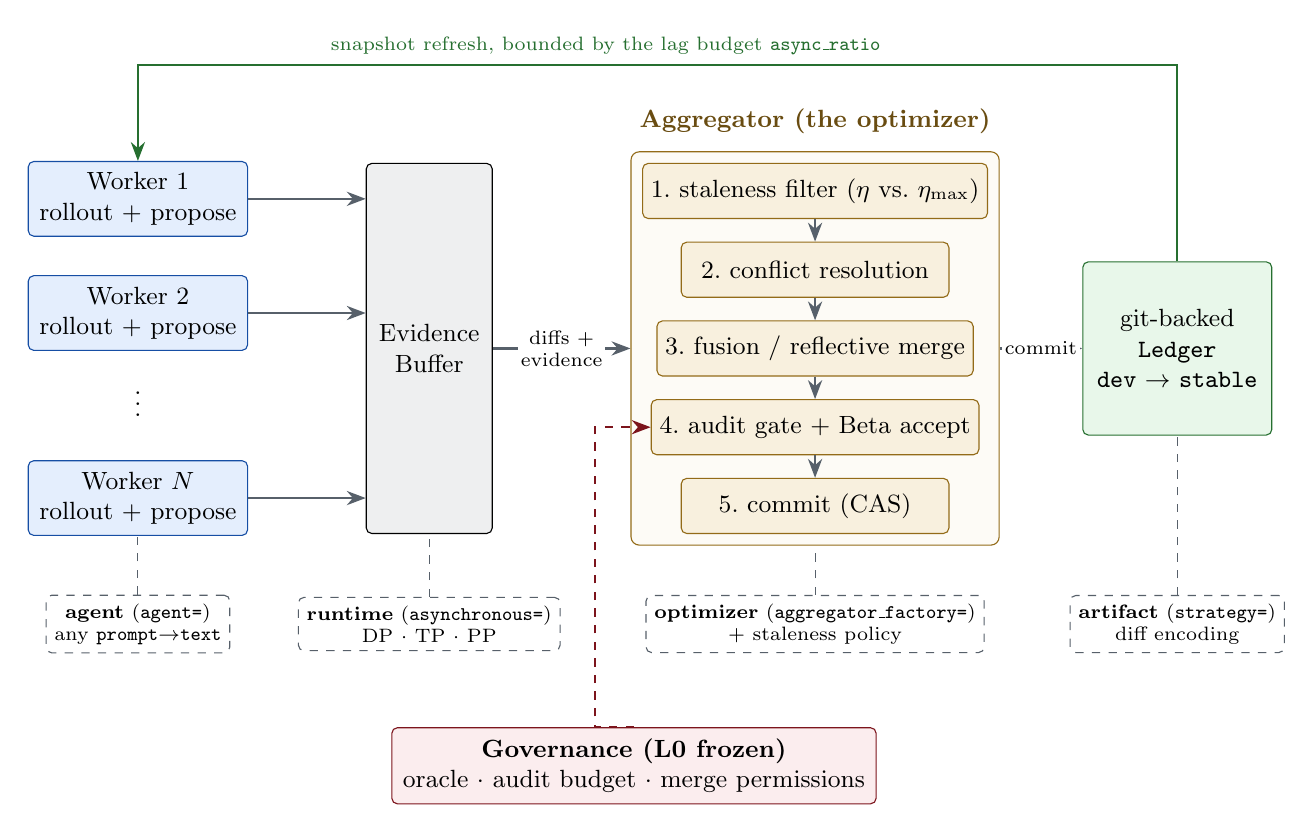
\begin{tikzpicture}[
  font=\small,
  box/.style={draw, rounded corners=2pt, align=center, minimum height=9mm, inner sep=4pt},
  worker/.style={box, fill=adblue!12, draw=adblue!70!black, minimum width=26mm},
  agg/.style={box, fill=adorange!15, draw=adorange!70!black, minimum width=34mm, minimum height=7mm, inner sep=3pt},
  ledger/.style={box, fill=adgreen!12, draw=adgreen!60!black, minimum width=24mm},
  gov/.style={box, fill=adred!8, draw=adred!60!black, align=center},
  seam/.style={draw=adgray, dashed, rounded corners=2pt, align=center, font=\scriptsize, inner sep=3pt, fill=white},
  arr/.style={-{Stealth[length=2.4mm]}, thick, adgray},
  elab/.style={font=\scriptsize, align=center, fill=white, inner sep=1pt},
]
% ---- row 1: the fixed data path ----
\node[worker] (w1) at (0, 1.9)  {Worker 1\\rollout + propose};
\node[worker] (w2) at (0, 0.45) {Worker 2\\rollout + propose};
\node          at (0,-0.6) {$\vdots$};
\node[worker] (wn) at (0,-1.9)  {Worker $N$\\rollout + propose};
\node[box, fill=adgray!10, minimum height=47mm, minimum width=16mm] (buf) at (3.7, 0) {Evidence\\Buffer};
\node[agg] (stale)  at (8.6, 2.0)  {1.\ staleness filter ($\eta$ vs.\ $\eta_{\max}$)};
\node[agg] (conf)   at (8.6, 1.0)  {2.\ conflict resolution};
\node[agg] (fuse)   at (8.6, 0.0)  {3.\ fusion / reflective merge};
\node[agg] (gate)   at (8.6,-1.0)  {4.\ audit gate + Beta accept};
\node[agg] (commit) at (8.6,-2.0)  {5.\ commit (CAS)};
\begin{scope}[on background layer]
\node[draw=adorange!70!black, rounded corners=3pt, fit=(stale)(commit), inner sep=4pt, fill=adorange!4] (aggbox) {};
\end{scope}
\node[above=1mm of aggbox, adorange!50!black, font=\small\bfseries] {Aggregator (the optimizer)};
\node[ledger, minimum height=22mm] (led) at (13.2, 0) {git-backed\\\code{Ledger}\\\code{dev} $\to$ \code{stable}};

\draw[arr] (w1.east) -- (buf.west |- w1.east);
\draw[arr] (w2.east) -- (buf.west |- w2.east);
\draw[arr] (wn.east) -- (buf.west |- wn.east);
\draw[arr] (buf.east) -- (aggbox.west);
\node[elab] at ($(buf.east)!0.5!(aggbox.west)$) {diffs +\\evidence};
\draw[arr] (aggbox.east) -- (led.west);
\node[elab] at ($(aggbox.east)!0.5!(led.west)$) {commit};
\draw[arr] (stale) -- (conf);  \draw[arr] (conf) -- (fuse);
\draw[arr] (fuse) -- (gate);   \draw[arr] (gate) -- (commit);

% ---- row 2: the seams, one per component ----
\node[seam] (sagent) at (0,-3.5)   {\textbf{agent} (\code{agent=})\\any \code{prompt$\to$text}};
\node[seam] (srun)   at (3.7,-3.5) {\textbf{runtime} (\code{asynchronous=})\\DP $\cdot$ TP $\cdot$ PP};
\node[seam] (sopt)   at (8.6,-3.5) {\textbf{optimizer} (\code{aggregator\_factory=})\\+ staleness policy};
\node[seam] (sart)   at (13.2,-3.5){\textbf{artifact} (\code{strategy=})\\diff encoding};
\draw[dashed, adgray] (sagent.north) -- (0,-2.35);
\draw[dashed, adgray] (srun.north)   -- (3.7,-2.35);
\draw[dashed, adgray] (sopt.north)   -- (8.6,-2.5);
\draw[dashed, adgray] (sart.north)   -- (13.2,-1.1);

% ---- row 3: the one layer that is not a seam, wired to the gate it governs ----
\node[gov] (govn) at (6.3,-5.3) {\textbf{Governance (L0 frozen)}\\oracle $\cdot$ audit budget $\cdot$ merge permissions};
% routed relative to the aggregator's own west edge, so it clears the box
% whatever width the stage labels give it
\path (aggbox.west) ++(-0.45,0) coordinate (glane);
\draw[arr, adred!60!black, dashed]
  (govn.north) -- (glane |- govn.north) -- (glane |- gate.west) -- (gate.west);

% ---- row 4: the single feedback edge, in its own lane ----
\draw[arr, adgreen!60!black]
  (led.north) -- (13.2,3.6) --
  node[above, font=\scriptsize, pos=0.55] {snapshot refresh, bounded by the lag budget \code{async\_ratio}}
  (0,3.6) -- (w1.north);
\end{tikzpicture}
\caption{AgentDescent architecture. \textbf{Solid, top:} the fixed data path --- $N$ workers roll out tasks against ledger snapshots and emit diffs with evidence cards into a thread-safe buffer; a dedicated aggregator thread runs the five-stage merge pipeline and commits winners to the git-backed ledger; the green return edge is the only feedback path, bounded by the lag budget. \textbf{Dashed, bottom:} the pluggable seams of \cref{sec:pluggable}, each selected by one keyword argument of \evolve{}. \textbf{Red:} the frozen L0 governance layer, deliberately not a seam.}
\label{fig:architecture}
\end{figure}

\subsection{System components}
\Cref{tab:analogy} summarizes the correspondence and \cref{fig:architecture} the resulting architecture. The \textbf{ledger} is the parameter server: a git-backed store with per-artifact version vectors, compare-and-swap (CAS) commits, and a dual \code{dev}/\code{stable} branch pair; \code{stable} is promoted after $K$ regression-free rounds on \code{dev}, an EMA-style confirmation in which a new commit restarts the counter. \textbf{Workers} hold snapshots of the library, roll out tasks, and emit (diff, evidence) pairs into a thread-safe buffer. The \textbf{aggregator} consumes the buffer and performs merge decisions (\cref{sec:aggregator}). Version vectors make the staleness of any diff computable at merge time:
\begin{equation}
\label{eq:eta}
\eta(d) \;=\; \max_{a \,\in\, \mathrm{touched}(d)} \bigl( v_{\mathrm{head}}(a) - v_{\mathrm{base}}(a) \bigr).
\end{equation}

\subsection{Pluggable seams}
\label{sec:pluggable}
Each component in \cref{fig:architecture} sits behind an explicit interface, selected by one keyword argument of the single entry point \evolve{}: the \emph{agent layer} (any $\code{prompt} \to \code{text}$ callable is a completion --- Claude, OpenAI-compatible endpoints, a tool-using CLI agent, or plain \code{run}/\code{reward}/\code{propose} functions), the \emph{strategy} (diff encoding), the \emph{aggregator} (\code{aggregator\_factory}), the \emph{staleness policy}, the \emph{runtime} (synchronous or barrier-free), the \emph{parallelism scheme} (data/tensor/pipeline \citep{shoeybi2019megatron,huang2019gpipe}; only the data-parallel path is exercised by any experiment here), and the \emph{executor and sandbox}. Selection and acceptance rules are likewise named policy classes. \Cref{sec:ports} uses these seams to port eighteen published algorithms without modifying the engine. The single deliberate exception is governance (\cref{sec:governance}): the L0 layer exposes no seam, since a self-modifying system must not be able to replace its own evaluator.

\section{The Aggregator as a Discrete-Space Optimizer}
\label{sec:aggregator}

Evidence cards are bucketed per artifact; when a bucket reaches batch size $B$ (or a timeout, so cold artifacts are not starved), the aggregator executes one optimizer step, summarized in \cref{alg:async}: \textbf{(1) staleness filtering} by \cref{eq:eta} under the active policy (\cref{sec:async}); \textbf{(2) conflict resolution} --- syntactic (overlapping hunks) and semantic (contradictory operations) conflicts are detected, and contradictions are resolved by \emph{dropping} the weaker member of each pair on a shared held-out subset. We name this conflict-drop rather than projection: PCGrad \citep{yu2020pcgrad} exists precisely to \emph{avoid} discarding a conflicting update, projecting it onto the normal plane so its non-conflicting component survives. Retaining the loser's non-conflicting keys would be the faithful analogue and is not implemented; \textbf{(3) fusion} --- complementary survivors are merged into one union candidate --- a union over disjoint keys, closer to disjoint task-vector merging than to the weight averaging of model soups \citep{wortsman2022modelsoups}, since nothing here is averaged, with \emph{reflective merge} handling contradictions that a keyed union cannot (\cref{sec:lever-val}); \textbf{(4) auditing} --- merges with high blast radius or low trust are routed through an oracle with veto power; \textbf{(5) statistical acceptance and commit}. Let $(s_c, f_c)$ and $(s_b, f_b)$ be the candidate's and the incumbent's successes and failures on the held-out split $\Dval$. The candidate commits (by CAS on \code{dev}) iff
\begin{equation}
\label{eq:accept}
\Pr\!\left[\theta_c > \theta_b\right] \;>\; 1 - \delta_v
\quad\textbf{and}\quad \hat r_c \ge \hat r_b,
\qquad
\theta_b \sim \mathrm{Beta}(1 + \pi_s + s_b,\; 1 + \pi_f + f_b),
\end{equation}
\begin{equation}
\label{eq:acceptcand}
\theta_c \sim \mathrm{Beta}\Bigl(1 + \pi_s + s_c + \textstyle\sum_j w_j \mathbb{1}[\delta_j > 0],\;\;
                                 1 + \pi_f + f_c + \textstyle\sum_j w_j \mathbb{1}[\delta_j \le 0]\Bigr),
\qquad w_j = \min(1, 4|\delta_j|).
\end{equation}
Three details of the released implementation are easy to elide and we state them because each is load-bearing. First, $(\pi_s, \pi_f)$ is a \emph{shared, running, per-artifact} prior rather than a uniform one: it accumulates over the run, absorbing each rejected candidate's observed delta and each commit as strong positive evidence, which is what makes the test conservative on artifacts with a history of failed edits. Second, the sum in \cref{eq:acceptcand} is applied to the \emph{candidate only}: each contributing evidence card folds its own before/after delta $\delta_j$ in as a pseudo-count, so a proposal that measurably helped its own rollout enters the gate with more weight than one that did not. This is an asymmetry in the candidate's favour and it has no counterpart on the incumbent. Third, the posterior test is \textbf{and}ed with a hard point threshold: a candidate whose full held-out rate $\hat r_c$ falls below the incumbent's is rejected outright regardless of the posterior. On the small held-out splits used here the point threshold, not the posterior, is frequently the binding constraint --- so the mechanism is a posterior test \emph{guarded by} a regression check, not a posterior test instead of a threshold. The probability is estimated by Monte Carlo. Both posteriors are sampled independently even though $s_b$ and $s_c$ come from evaluating the two artifacts on the \emph{same} $\Dval$; a paired test would use that pairing and we do not, which makes the comparison noisier than it needs to be. The confidence requirement $\delta_v$ is annealed over the artifact's version $v$ (the learning-rate-decay analogue) and a trust region caps diff size.

One risk of this discipline deserves explicit statement: the gate reuses a single fixed $\Dval$ across many acceptance decisions (hundreds of proposals per run in \cref{sec:exp-ports}), so accepted diffs are selected extreme statistics on $\Dval$ and their measured gains are optimistically biased --- the standard adaptive-data-analysis concern. Two mitigations are in place and one is not: all quality results in \cref{sec:experiments} are reported on a disjoint \emph{test} split the gate never sees; the trust region and annealed $\delta_v$ limit how much any single decision can exploit $\Dval$; but no reusable-holdout or $\Dval$-rotation mechanism is implemented. We therefore measure the resulting bias directly (\cref{sec:exp-ports}): across 33 runs the gain the gate observed on $\Dval$ exceeds the gain realized on test by $0.038$ on average, a small but statistically detectable optimism that a reader should subtract from any $\Dval$-reported figure.

A natural objection to merge-based evolution is that two individually beneficial edits may be jointly harmful. Two properties bound the risk: the acceptance test \cref{eq:accept} scores the \emph{fused} candidate on the full held-out split, so a harmful fusion cannot commit under the single merger used here (the rebase path in \code{\_commit\_with\_retry} does not re-run acceptance, so this guarantee would need restating for multi-merger operation); and the union is a superset of the diffs that survive conflict resolution --- which drops the weaker member of each contradicting pair first, so it is not a superset of every proposal. An optional \emph{fusion tournament} additionally ranks the union against its constituents; it is disabled by default (it costs one additional held-out sweep per candidate against a recoverable gain) but serves as the measurement instrument for the objection, reporting win rate, the losing tail, and a \code{contested} counter that records whether a fused candidate was in fact constructed and ranked --- so a run in which fusion never occurred cannot be reported as a merge win. \Cref{sec:merge-vs-fork} reports the win rate in situ for one workload; we attach no headline to it, because it is a property of that artifact's key granularity and proposal overlap rather than of the mechanism.

\section{Efficiency Analysis: Three Sources of Speedup}
\label{sec:efficiency}

Wall-clock time in a self-evolution loop decomposes into rollout time, synchronization time, and held-out validation time. AgentDescent addresses each with a distinct mechanism; the third is specific to merge-based evolution.

\subsection{Overlapping I/O-bound rollouts}
\label{sec:concept-parallel}
Agent rollouts are dominated by time spent waiting on a model endpoint, so thread-level concurrency suffices to overlap them (\cref{sec:exp-parallel} measures $5.8\times$ at eight threads on real API calls). The synchronous data-parallel runtime shards tasks across $N$ workers over a common snapshot and merges at a round barrier. The barrier, however, imposes a ceiling independent of $N$: with i.i.d.\ rollout latencies $t_i$,
\begin{equation}
\label{eq:barrier}
T_{\mathrm{round}}^{\mathrm{sync}} \;=\; \mathbb{E}\bigl[\max_{i \le N} t_i\bigr] \;+\; T_{\mathrm{gate}},
\end{equation}
and reasoning-model latencies are heavy-tailed --- a short answer and a long deliberation are the same call --- which maximizes the gap between $\mathbb{E}[\max_i t_i]$ and $\mathbb{E}[t]$. The second term is a serial region in which all workers idle while the gate evaluates.

\subsection{Barrier-free execution under bounded staleness}
\label{sec:async}
The asynchronous runtime (\cref{alg:async}) removes the round structure: workers produce continuously, a dedicated merger consumes continuously, and per-rollout cost approaches $\mathbb{E}[t]$ --- the no-barrier discipline of asynchronous RL systems \citep{fu2025areal,roll2025flash} transferred to self-evolution. Its cost is staleness, which \cref{eq:eta} makes first-class and per-diff, bounded by two mechanisms. A \emph{lag budget} $\rho$ (\code{async\_ratio}) limits drift at the source: a worker refreshes its snapshot once $v_{\mathrm{head}}$ exceeds its snapshot version by more than $\rho$, and backpressure forces a global resynchronization if evidence accumulates while nothing commits. A \emph{staleness policy} disposes of stale diffs at the merger: \textsc{Full} admits them unconditionally (sound only where diffs compose); \textsc{Guarded} rebases within $\eta \le \eta_{\max}$ and discards beyond, in the spirit of bounded-staleness RL \citep{fu2025areal}, paying for safety in discarded rollouts; \textsc{Reflective} always rebases and \emph{re-verifies} --- a stale diff is treated as unproven rather than invalid, and is discarded only if its claimed improvement fails to hold on the new head. Because $\rho$ is denominated in artifact versions, its appropriate value scales with rollout cost; the runtime emits a warning when a run discards the majority of its evidence.

\begin{algorithm}[t]
\caption{Barrier-free evolution (\code{async\_evolve}); the synchronous runtime is the special case with a round barrier between the two loops. $S$ is the strategy of \cref{sec:setup}. Backpressure has two parts: \code{buffer.put} blocks while the un-merged intake exceeds the lag budget, and a stall detector (evidence arriving while nothing commits) forces a global resynchronization. In the current implementation a single merger thread performs all commits, so the CAS never contends; multi-merger operation, where it would, is future work.}
\label{alg:async}
\begin{algorithmic}[1]
\State \textbf{Worker $i$ (in parallel, $i = 1..N$):}
\Loop
  \If{$v_{\mathrm{head}} - v_i > \rho$} refresh snapshot $A_i \gets$ ledger head; $v_i \gets v_{\mathrm{head}}$ \EndIf
  \State sample task $x$; rollout $\tau \gets \pi_{A_i}(x)$; reward $r \gets r(\tau, x)$
  \State $(d, e) \gets S.\mathrm{propose}(A_i, x, \tau, r)$; \; buffer.put$(d, e)$ \Comment{blocks on backpressure}
\EndLoop
\State \textbf{Merger (single thread):}
\Loop
  \State $\mathcal{B} \gets$ buffer.drain(); bucket $\mathcal{B}$ by artifact
  \For{each bucket with $|\mathcal{B}_a| \ge B$ or timed out}
    \State $\mathcal{B}_a \gets \{\, d : \mathrm{policy}(\eta(d), \eta_{\max}) \ne \textsc{discard} \,\}$, rebasing where directed \Comment{\cref{eq:eta}}
    \State resolve conflicts (keep better of each contradicting pair); $u \gets \mathrm{fuse}(\text{survivors})$
    \Statex \hskip\algorithmicindent \textit{(with reflective merge the conflict policy is replaced too:}
    \Statex \hskip\algorithmicindent \textit{contradictions are kept rather than resolved, and $u \gets$ model-written union)}
    \If{audit passes \textbf{and} \cref{eq:accept} holds on $\Dval$} CAS-commit $u$ to \code{dev} \EndIf
  \EndFor
  \State promote \code{dev} $\to$ \code{stable} after $K$ regression-free rounds
\EndLoop
\end{algorithmic}
\end{algorithm}

\subsection{Reducing validation cost}
\label{sec:lever-val}
The third source of speedup is unavailable to the first two mechanisms: the gate itself. Every acceptance decision costs one sweep over $\Dval$, and on live models this dominates the merger's critical path: profiled on a live GEPA/HotpotQA run ($N{=}4$, \code{GLM-5.2}), the merger thread is busy $560.1$\,s of a $740$\,s process --- $75.7\%$ occupancy on a single thread. We report the occupancy and not a gate/non-gate split: in the released instrumentation the two timers wrap the same region, so their ratio is $1.0$ by construction rather than by measurement, and a decomposition of the merger's time into evaluation, ledger I/O and commit needs instrumentation this paper does not have. A serial or selection-based loop with $m$ proposals pays $m \cdot |\Dval|$ gate evaluations. Merging changes the count: a round's $k$ surviving diffs fuse into one candidate, so per-round gate cost falls from $k \cdot |\Dval|$ to $|\Dval|$; a diff discarded by the staleness filter never reaches the gate and costs zero evaluations; and in the asynchronous runtime, cards arriving during a merge enlarge the next batch rather than triggering additional merges. The effect is visible directly in the RQ1 experiment (\cref{fig:mspr}): model-seconds per rollout fall across the serial, synchronous, and asynchronous arms at a pinned rollout budget. Two costs partially offset the saving and are stated for balance: the \textsc{Reflective} staleness policy's re-verification spends additional gate evaluations, and a model-written reflective merge spends one further model call per contested fusion. Residual gate cost parallelizes independently of the worker pool (\code{eval\_concurrency}), saturating at $|\Dval|$.

The reduction presupposes that proposals \emph{can} fuse, which fails exactly when the artifact's key space is too coarse. An artifact held in a single key --- e.g.\ a prompt as one instruction slot, GEPA's setting \citep{agrawal2025gepa} --- makes every pair of concurrent proposals a write--write conflict; a keyed union then degenerates to retaining the better single proposal, i.e.\ best-of-$n$ selection at best-of-$n$ validation cost. \emph{Reflective merge} restores the reduction: a model is prompted to write the \emph{union} of the contradicting proposals --- one candidate preserving each proposal's intent --- and the union passes through the same acceptance test as any candidate, so the model proposes and the gate decides. \Cref{sec:exp-reflective} measures what this is worth on a one-key artifact, where nothing else can fuse. Key granularity is necessary but not sufficient, and the missing condition is quantifiable. The engine proposes only from a rollout that \emph{failed} --- a solved task yields no diff --- so if the incumbent fails a fraction $f$ of tasks and $N$ workers run per round, the probability that a round produces at least two diffs, and therefore anything to fuse, is
\begin{equation}
\label{eq:fusionrate}
P_{\text{fuse}}(f, N) \;=\; 1 - (1-f)^N - N f (1-f)^{N-1}.
\end{equation}
This is a \emph{necessary} condition and an upper bound, not a prediction of the fusion rate, and the gap between the two is large enough to state plainly. \Cref{eq:fusionrate} counts rounds with two failed rollouts; between a failed rollout and a diff in the aggregator's bucket sit several further filters that it ignores --- the proposer can return nothing, the strategy can fail to encode a proposal as a diff, the staleness filter can discard, and the aggregator buckets \emph{per artifact}, so two failures touching different artifacts produce nothing to fuse. Measured against the runs of \cref{sec:merge-vs-fork}, where $f \approx 0.9$ puts the bound at essentially $100\%$: at $N{=}8$ the aggregator contested $10$ of $24$ rounds ($42\%$) and at $N{=}4$, $21$ of $144$ ($15\%$) --- the bound overpredicts by $2.4\times$ and $6.8\times$. So \cref{eq:fusionrate} is useful in one direction only: when it is \emph{small}, merging cannot fire and no experiment on that workload can measure merging, which is exactly how it retrodicts our two nulls. When it is large, merging may still rarely fire, and only the \code{contested} counter settles it. A near-saturated artifact starves the merge step no matter how finely its keys are cut; a far-from-saturated one merely permits fusion. \Cref{sec:merge-vs-fork} measures both sides of it. It is the spatial counterpart of the \textsc{Reflective} staleness policy (carry intent onto a changed base; let measurement decide), and the \code{contested} counter reports whether fusion genuinely occurred, so the saving is never claimed where only selection took place.

\begin{figure}[t]
\centering
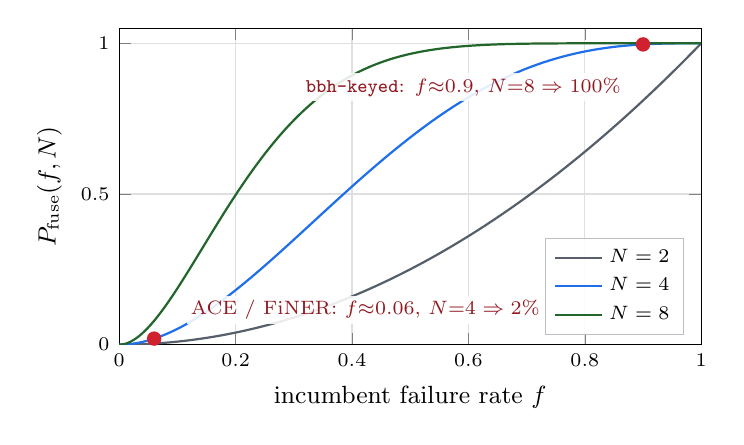
\begin{tikzpicture}
\begin{axis}[
  width=0.74\textwidth, height=5.6cm,
  xlabel={incumbent failure rate $f$},
  ylabel={$P_{\mathrm{fuse}}(f,N)$},
  domain=0:1, samples=201,
  xmin=0, xmax=1, ymin=0, ymax=1.05,
  grid=major, grid style={adgray!20},
  legend pos=south east,
  legend style={font=\scriptsize, draw=adgray!40, fill=white, fill opacity=0.9, text opacity=1},
  tick label style={font=\scriptsize}, label style={font=\small},
]
\addplot[thick, adgray]            {1-(1-x)^2-2*x*(1-x)};    \addlegendentry{$N=2$}
\addplot[thick, adblue]            {1-(1-x)^4-4*x*(1-x)^3};  \addlegendentry{$N=4$}
\addplot[thick, adgreen!55!black]  {1-(1-x)^8-8*x*(1-x)^7};  \addlegendentry{$N=8$}
\addplot[only marks, mark=*, mark size=2.4pt, adred] coordinates {(0.06,0.020) (0.90,0.9963)};
\node[font=\scriptsize, anchor=west, adred!70!black, fill=white,
      fill opacity=0.88, text opacity=1, inner sep=1.5pt] at (axis cs:0.115,0.115)
  {ACE / FiNER: $f{\approx}0.06$, $N{=}4 \Rightarrow 2\%$};
\node[font=\scriptsize, anchor=east, adred!70!black, fill=white,
      fill opacity=0.88, text opacity=1, inner sep=1.5pt] at (axis cs:0.87,0.855)
  {\code{bbh-keyed}: $f{\approx}0.9$, $N{=}8 \Rightarrow 100\%$};
\end{axis}
\end{tikzpicture}
\caption{The fusion precondition of \cref{eq:fusionrate}: the fraction of rounds in which at least two diffs exist, and therefore anything to fuse at all. Because the engine proposes only from \emph{failed} rollouts, a near-saturated artifact starves the merge step regardless of how finely its keys are cut --- the curve collapses at small $f$ for every width. Red markers are the two workloads of \cref{sec:merge-vs-fork}: the one whose merge step never fired sits at $2\%$, and the one built to satisfy the condition sits at $100\%$. Widening $N$ moves the curve left, which is how the equation bounds fusion width \emph{from below}; the round count and the trust region bound it from above.}
\label{fig:fusionrate}
\end{figure}

\section{Governance by Blast Radius}
\label{sec:governance}

Artifacts are assigned to layers by a declared \code{blast\_radius}: \textbf{L2} (skills, prompts) merges under the full asynchronous pipeline, \textbf{L1} (harnesses, verifiers) serializes and routes every merge through the oracle, and \textbf{L0} (the oracle, audit budget, merge permissions) is frozen and read-only to the loop --- deliberately the one component with no pluggable seam, since a self-referential loop that can replace its own verifier converges to one that accepts its own output. Executed agent code runs behind a frozen test suite overlaid after workspace materialization. This is a design position, not a result: no experiment in this paper attacks it.

\section{Case Study: Porting Eighteen Self-Evolution Algorithms}
\label{sec:ports}

Because every component sits behind a seam (\cref{sec:pluggable}), porting a published algorithm requires a small set of plug-ins rather than a fork. Two routes cover all eighteen ports.

\paragraph{Route 1: a strategy, plus an optimizer where needed.} A \emph{benchmark-faithful} port supplies a \code{strategy} encoding the paper's artifact as keyed diffs and, only when its search differs from the default pipeline, an \code{aggregator\_factory}. The seven faithful ports illustrate the scale of the required code: ACE \citep{zhang2025ace} is a playbook strategy whose curator \emph{is} the default aggregator; GEPA \citep{agrawal2025gepa} substitutes a per-instance Pareto optimizer; ADAS \citep{hu2024adas} and DGM \citep{zhang2025dgm} plug in keep-all archives with their own parent selection; EvoSkill a bounded top-$K$ frontier; SkillOpt a strict edit gate;\footnote{EvoSkill and SkillOpt are ports of released systems whose upstream papers and per-port departures are identified in the repository's port-fidelity documentation; we do not cite them here to avoid attributing a reconstruction to the wrong reference.} OpenEvolve \citep{openevolve2025} MAP-Elites islands \citep{mouret2015mapelites}. Parent-selection and acceptance rules are extracted as named policy classes, so subsequent ports reuse them.

\paragraph{Route 2: a declarative policy bundle.} The eleven microports and analogues (PromptBreeder, AFlow, Self-Refine, Reflexion, SICA, G\"odel Agent, Voyager, SkillWeaver, Absolute Zero, R-Zero, Agent0) define no new classes: each is a \code{MethodPolicy} --- selection rule, memory, acceptance shape, genome --- over one shared runner, inheriting a common budget contract, dataset layer, and command line. A shared \code{-{}-serial} flag reproduces the upstream algorithm's own semantics (one worker, serial gate) as the control that any parallelization claim requires, and a shared rollout budget pins compared arms to equal work.

Fidelity is declared per port --- \emph{benchmark-faithful}, \emph{mechanism microport}, \emph{self-edit analogue}, \emph{environment analogue}, or \emph{inference analogue} --- follows the released code where it diverges from the paper, and documents infrastructure boundaries explicitly; analogues are not to be cited as benchmark reproductions. All eighteen ports run under serial, synchronous, and barrier-free scheduling without modification, which is what makes the scheduler a controlled variable rather than a property of each paper's own loop.

\section{Evaluation}
\label{sec:experiments}

\paragraph{Setup.} All results are obtained from live models on real datasets: \code{deepseek-v4-flash} and \code{GLM-5.2} (reasoning models) via an OpenAI-compatible endpoint, on each algorithm's own benchmark. Every number is produced by a named script in the repository with its exact reproduction command; absolute times depend on host and endpoint, so ratios are the reproducible quantity. We address four questions: \textbf{RQ1} --- how much effective concurrency do the three mechanisms of \cref{sec:efficiency} deliver against a faithful serial control? \textbf{RQ2} --- what does reflective merge buy, on an artifact where nothing else can fuse? \textbf{RQ3} --- is learning behavior preserved under the most aggressive schedule, and how optimistic is the gate that decides it? \textbf{RQ4} --- does merging accelerate without a quality penalty relative to best-of-$N$ selection at equal budget?

\paragraph{Statistical conventions.} Spreads across seeds are sample standard deviations. Sign tests are exact and two-sided with ties dropped, and the unit of analysis is stated with each one. No correction for multiple comparisons is applied anywhere; the paper makes on the order of a hundred pairwise comparisons, so a single nominal $p$ near $0.05$ should be read as descriptive. Where a design cannot reach significance --- which is the case for every RQ4 quality comparison --- we report paired confidence intervals and the minimum detectable effect instead of a $p$-value.

\Cref{tab:config} states every configuration in full, including the two runs that produced null results and are reported as such. Three conventions hold throughout and are worth stating once, because each of them costs us something. The rollout budget is \emph{pinned on every arm} of every comparison, so a wide arm cannot buy its speedup with extra work --- the failure mode that makes an unbudgeted $N{=}8$ arm look eight times better. The serial control runs its gate at \code{eval\_concurrency}${=}1$, reproducing the published loop rather than a partly-parallel version of it; this makes the control slower and every speedup beside it larger, which is why the value is recorded rather than assumed. And the held-out \emph{test} split is disjoint from the gate's $\Dval$ in every experiment, so no quality figure below was ever seen by an acceptance decision.

\begin{table}[t]
\centering
\footnotesize
\setlength{\tabcolsep}{4pt}
\caption{Every configuration behind \cref{sec:experiments}. Budget is pinned in rollouts on all arms of a comparison unless noted. Flags not listed take each script's defaults, which every run prints in its header and records in its result JSON; \cref{sec:repro} names the script per experiment. Model names are the endpoint's identifiers.}
\label{tab:config}
\begin{tabular}{@{}>{\raggedright\arraybackslash}p{1.95cm}>{\raggedright\arraybackslash}p{1.95cm}>{\raggedright\arraybackslash}p{2.6cm}>{\raggedright\arraybackslash}p{1.7cm}>{\raggedright\arraybackslash}p{2.05cm}>{\raggedright\arraybackslash}p{3.8cm}@{}}
\toprule
\textbf{Experiment} & \textbf{Model} & \textbf{Workload} & \textbf{Arms, width} & \textbf{Budget, seeds} & \textbf{Gate, staleness, notes} \\
\midrule
Thread overlap (\cref{sec:exp-parallel})
& \code{GLM-5.2}
& 8 concurrent API calls of matched request length
& 8 threads vs.~1
& 3 repeats
& Pure-Python CPU work run through the same harness as the GIL control \\
\addlinespace
RQ1 (\cref{sec:exp-live})
& \code{GLM-5.2}
& HotpotQA via the GEPA port; \code{-{}-fetch 80}, \code{-{}-val-cap 8}
& serial / sync / async, $N{=}4$
& 16 rollouts per arm; seeds 0--2
& Gate at \code{eval\_concurrency}${=}16$ on the parallel arms, ${=}1$ on the serial control; \code{-{}-async-ratio 3}; \code{-{}-rounds 9999} so the budget binds, not the port's own iteration default; \code{-{}-reflective-merge} on \emph{every} arm, so it is not a difference between them; reasoning tokens disabled \\
\addlinespace
RQ3 (\cref{sec:exp-ports})
& \code{deepseek-}\allowbreak\code{v4-flash}
& each port's own benchmark, 11 ports
& barrier-free only, $N{=}8$
& 80 rollouts per seed; seeds 0--2
& \textsc{Full} staleness, the most permissive policy --- stale diffs admitted unconditionally; 465--2{,}069 model calls per seed \\
\addlinespace
RQ4, null 1 (\cref{sec:merge-vs-fork})
& \code{GLM-5.2}
& HotpotQA; artifact is a single instruction slot
& serial / fork / merge, $N{=}3$
& 9 rollouts per seed; seeds 0--2
& Reflective merge on. 1{,}298 calls, 11.3\,h model time. Reported as a null: the fused union was built twice in the whole experiment \\
\addlinespace
RQ4, null 2 (\cref{sec:merge-vs-fork})
& \code{GLM-5.2}
& FiNER-139 via the ACE playbook, keyed per bullet; \code{-{}-pool 2000}, \code{-{}-val-cap 32}
& serial / fork / merge, $N{=}4$
& 24 rollouts; seed 0
& Reflective merge and fusion tournament on. Reported as a null, and \cref{eq:fusionrate} explains it: the seed artifact already scored $0.938$ on the gate's split, so $f \approx 0.06$ \\
\addlinespace
RQ2 (\cref{sec:exp-reflective})
& \code{GLM-5.2}
& BBH \code{dyck\_languages} behind an \code{InstructionSlot} --- \emph{one} key; \code{-{}-fetch 120}, 60 train / 30 val / 30 test
& merge only, $N{=}4$
& 48 rollouts per arm; seeds 0--3
& Three configurations: \textsc{Base} is the engine's shipped defaults, \textsc{Off} adds \code{-{}-fusion-tournament}, \textsc{On} is \code{-{}-reflective-merge}, which installs \code{KeepContradictions} as well as \code{ReflectiveFusion}. \textsc{Base} and \textsc{On} differ in the conflict policy and the fusion policy. Self-verification on in both. 9{,}828 calls across the three configurations, 20.3\,h model time \\
\addlinespace
RQ4, width 8 (\cref{sec:merge-vs-fork})
& \code{GLM-5.2}
& \code{bbh-keyed}: BBH \code{dyck\_languages} crossed with \code{KeyedRules}; 60 train / 30 val / 30 test
& serial / fork / merge, $N{=}8$
& 32 rollouts per arm (4 rounds); seeds 0--5
& Keyed union (\code{DefaultFusion}) with the fusion tournament and self-verification on; \emph{not} reflective merge --- \code{ReflectiveFusion} records every trial unranked, so the contested counts reported below could not exist under it. 16{,}124 calls, 28.3\,h model time \\
\addlinespace
RQ4, width 4 (\cref{sec:merge-vs-fork})
& \code{GLM-5.2}
& as above, same splits
& serial / fork / merge, $N{=}4$
& 96 rollouts per arm (24 rounds); seeds 0--5
& As above. The width matched to the trust region, at a $3\times$ budget so the round count rises rather than falls \\
\bottomrule
\end{tabular}
\end{table}

\subsection{RQ1: Effective concurrency against a faithful serial control}
\label{sec:exp-live}
\label{sec:exp-parallel}

\begin{figure}[t]
\centering
\begin{minipage}[t]{0.32\textwidth}
\centering
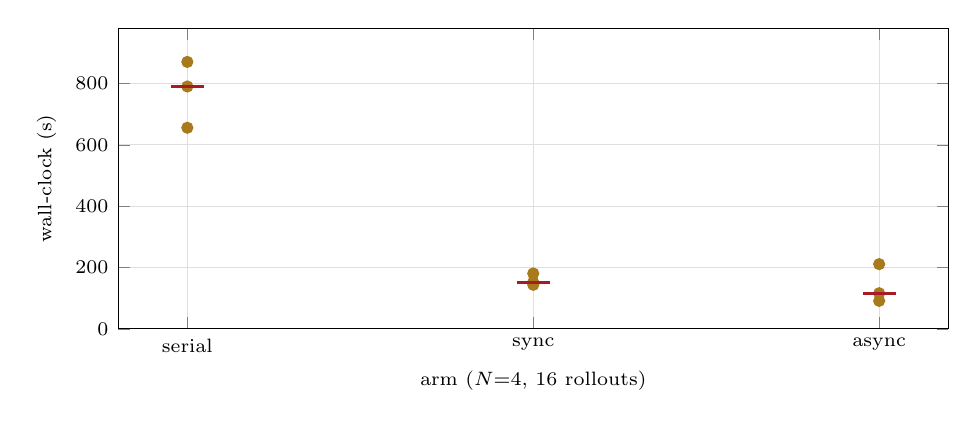
\begin{tikzpicture}
\begin{axis}[
  width=\textwidth, height=5.4cm,
  xlabel={arm ($N{=}4$, 16 rollouts)},
  ylabel={wall-clock (s)},
  symbolic x coords={serial, sync, async},
  xtick=data, ymin=0, ymax=980,
  grid=major, grid style={adgray!20},
  tick label style={font=\scriptsize}, label style={font=\scriptsize},
]
\addplot[only marks, mark=*, mark size=2pt, adorange!80!black] coordinates {
  (serial,655.6) (serial,870.2) (serial,790.1)
  (sync,180.6) (sync,143.6) (sync,152.1)
  (async,211.0) (async,91.3) (async,116.2)};
\addplot[only marks, mark=-, mark size=6pt, very thick, adred!80!black] coordinates {
  (serial,790.1) (sync,152.1) (async,116.2)};
\end{axis}
\end{tikzpicture}
\caption{RQ1, the quantity the framework exists to reduce: wall-clock to spend a pinned rollout budget. GEPA on HotpotQA, \code{GLM-5.2}, 16 rollouts on every arm, three seeds, medians marked. median $790 \to 152 \to 116$\,s: parallelism takes the first $5.2\times$, barrier removal a further $1.31\times$, $6.8\times$ end to end --- but the per-seed end-to-end ratios span $3.1$--$9.5\times$, so the median is a location, not a bound.}
\label{fig:wall}
\end{minipage}\hfill
\begin{minipage}[t]{0.32\textwidth}
\centering
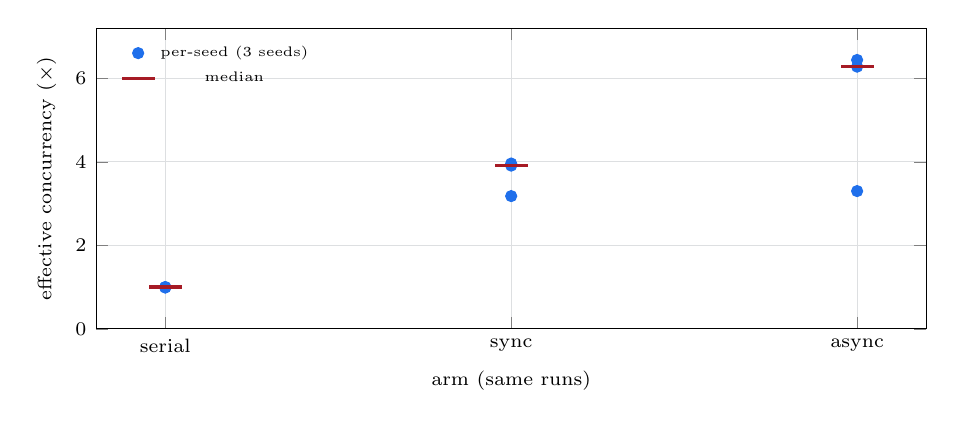
\begin{tikzpicture}
\begin{axis}[
  width=\textwidth, height=5.4cm,
  xlabel={arm (same runs)},
  ylabel={effective concurrency ($\times$)},
  symbolic x coords={serial, sync, async},
  xtick=data, ymin=0, ymax=7.2,
  grid=major, grid style={adgray!20},
  tick label style={font=\scriptsize}, label style={font=\scriptsize},
  legend style={font=\tiny, at={(0.02,0.98)}, anchor=north west, draw=none, fill=none},
]
\addplot[only marks, mark=*, mark size=2pt, adblue] coordinates {
  (serial,0.99) (serial,1.00) (serial,1.00)
  (sync,3.18) (sync,3.91) (sync,3.96)
  (async,3.30) (async,6.28) (async,6.44)};
\addlegendentry{per-seed (3 seeds)}
\addplot[only marks, mark=-, mark size=6pt, very thick, adred!80!black] coordinates {
  (serial,1.00) (sync,3.91) (async,6.28)};
\addlegendentry{median}
\end{axis}
\end{tikzpicture}
\caption{Where that time goes: effective concurrency (model-seconds $\div$ wall-clock). The serial control reproduces the published loop (one worker, serial gate) and lands at $0.99$--$1.00\times$ on every seed --- a stable control property, not a single-run coincidence. Synchronous parallelism spans $3.18$--$3.96\times$; barrier removal spans $3.30$--$6.44\times$, the widest arm, and reaches it while overrunning the pinned budget (19 rollouts against 16).}
\label{fig:concurrency}
\end{minipage}\hfill
\begin{minipage}[t]{0.32\textwidth}
\centering
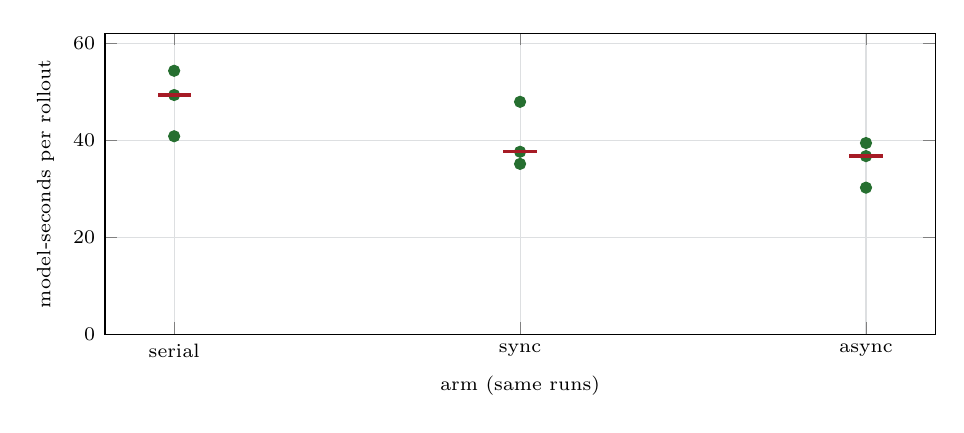
\begin{tikzpicture}
\begin{axis}[
  width=\textwidth, height=5.4cm,
  xlabel={arm (same runs)},
  ylabel={model-seconds per rollout},
  symbolic x coords={serial, sync, async},
  xtick=data, ymin=0, ymax=62,
  grid=major, grid style={adgray!20},
  tick label style={font=\scriptsize}, label style={font=\scriptsize},
]
\addplot[only marks, mark=*, mark size=2pt, adgreen!60!black] coordinates {
  (serial,40.8) (serial,54.3) (serial,49.3)
  (sync,47.9) (sync,35.1) (sync,37.6)
  (async,36.7) (async,30.2) (async,39.4)};
\addplot[only marks, mark=-, mark size=6pt, very thick, adred!80!black] coordinates {
  (serial,49.3) (sync,37.6) (async,36.7)};
\end{axis}
\end{tikzpicture}
\caption{Validation-cost reduction in the same runs (\cref{sec:lever-val}): model-seconds spent per rollout at a pinned rollout budget, per seed, with medians marked. The parallel arms evaluate less per unit of work --- median $49.3 \to 37.6 \to 36.7$ --- but the asynchronous figure is normalized by \emph{measured} rollouts, and that arm ran 19 against the pinned 16. Charged against the budget every arm was given, it is $36.7 \times 19/16 = 43.6$, above the synchronous arm's $37.6$: the serial-to-synchronous step survives the correction and the synchronous-to-asynchronous step does not. We cannot attribute this to any one cause. A \emph{keyed} union is never contested on a single-key slot, but \code{-{}-reflective-merge} is on in these arms, and \cref{sec:exp-reflective} shows that on exactly this artifact shape it does fuse and does cut calls --- so it is a live candidate here rather than an excluded one. The others are the admission cap (one merged candidate per round, so the Pareto pool grows by one instead of $N$) and, in principle, staleness discards --- though these runs record \code{stale\_discarded}${=}0$, which rules that one out. Separating the remaining two needs an arm without the cap, which we have not run.}
\label{fig:mspr}
\end{minipage}
\end{figure}

We first verify the premise of \cref{sec:concept-parallel}: eight threads over one pool reduce a real \code{GLM-5.2} API workload from 48.6\,s to 8.3\,s ($5.8\times$ in this run; 5.8--6.5$\times$ across three repeats, sub-linear under heavy-tailed latency), while the same threads on pure-Python CPU work yield $1.1\times$ --- rollout overlap is real, and the GIL does not limit I/O-bound rollouts.

The main experiment ports GEPA to its own benchmark (HotpotQA \citep{agrawal2025gepa,yang2018hotpotqa}) with 16 rollouts pinned on every arm, three seeds, and a control that reproduces the upstream loop exactly: one worker \emph{and} a serial gate. That control lands at $0.99$, $1.00$, and $1.00\times$ overlap on the three seeds (\cref{fig:concurrency}). We report it as a sanity check rather than as evidence: a one-worker arm whose gate scores one task at a time spends its life inside one blocking call, so a ratio near $1$ is close to arithmetic. What it confirms is that the control was configured as intended, not that it is a good control. Against it, synchronous parallelism spans $3.18$--$3.96\times$ effective concurrency (median $3.91$) and barrier removal spans $3.30$--$6.44\times$ (median $6.28$); median wall-clock falls $790 \to 152 \to 116$\,s (\cref{fig:wall}) --- a $6.8\times$ reduction in the time to spend the same rollout budget, which is the framework's core claim in its most direct form. \Cref{fig:mspr} shows model-seconds per rollout in the same runs: a median $49.3$ (serial), $37.6$ (synchronous), $36.7$ (asynchronous). It does not replicate cleanly --- one of three seeds contradicts each step (serial $40.8 \to$ synchronous $47.9$; synchronous $37.6 \to$ asynchronous $39.4$) --- the parallel arms not only finish sooner, they evaluate less per unit of work. Independent endpoint probes sustain $7\times$ (matched width and request length) to $10\times$ (wider, shorter requests) concurrency, so no arm is provider-limited.

Three qualifications bound these numbers. First, \emph{the asynchronous arm is not paying the same bill}: lacking a round boundary it ran 19 rollouts against the pinned 16 on every seed, so part of its concurrency is work the other arms did not perform. Second, \emph{it is also the least stable arm} --- a $3.30$--$6.44\times$ spread against synchronous parallelism's $3.18$--$3.96\times$. Third, and most important, \emph{none of this is a quality claim}: median held-out test score is $0.55$ (serial), $0.60$ (synchronous), $0.50$ (asynchronous) across the three seeds, on a 20-item split whose resolution is $0.05$, so the arms are indistinguishable in quality and the fastest arm is not the best one. One synchronous cell (seed 0) also ended early on an endpoint error at 12 of 16 rollouts and is included as measured.

These figures supersede a single-run measurement of $1.85\times / 3.22\times$ on a different model reported in an earlier draft. Two differences account for the gap and neither is a correction of the other: this run uses \code{GLM-5.2} rather than \code{deepseek-v4-flash}, and its parallel arms run the gate at \code{eval\_concurrency}${=}16$. The second is the more instructive: with the gate itself parallelized, the round barrier costs much less, which both raises the synchronous arm and shrinks what barrier removal has left to recover --- the regime dependence that decides when removing the barrier pays at all. An earlier draft additionally reported a width-8 variant with a 28\% model-call saving; it is withdrawn because its serial arm ran with a concurrent gate, violating the control definition above. The shipped cell for that run records 3849.7 model-seconds inside a 2148.4\,s wall-clock, i.e.\ $1.79\times$; an earlier draft quoted $1.31\times$ for the same cell and that figure was wrong.

\subsection{RQ2: What reflective merge buys, isolated}
\label{sec:exp-reflective}
The keyed union of \cref{sec:aggregator} fuses diffs that touch different keys. When an artifact is held in \emph{one} key, every pair of concurrent proposals is a write--write conflict, the union cannot be formed, and merge-of-$N$ collapses into best-of-$N$ selection. It also still pays to \emph{choose}: resolving a contradiction by comparison costs a held-out evaluation of each member of the pair, which is the cost this experiment turns out to measure. \emph{Reflective merge} is the mechanism that is supposed to close that gap: a model writes one value preserving what each proposal contributed, and the union goes through the same acceptance test as any other candidate. Everything said about it so far in this paper has been a design argument. This experiment measures it.

The workload is chosen so the mechanism is the \emph{only} thing that can fuse: BBH \code{dyck\_languages} \citep{suzgun2023bbh} behind an \code{InstructionSlot}, a one-key artifact on which a keyed union is never available. Two configurations, 48 rollouts pinned, $N{=}4$, four seeds, the same 60/30/30 split, the same gate. \textsc{Off} runs the keyed union with the fusion tournament enabled so the degeneracy is visible in the counters; \textsc{On} runs reflective merge. \emph{These differ in more than the fusion policy, and the difference matters for the cost column below.} \code{-{}-reflective-merge} installs a pair: \code{ReflectiveFusion} \emph{and} \code{KeepContradictions}, because a fusion policy installed alone is handed one diff --- conflict resolution runs first and has already discarded the contradictions it would have merged. So \textsc{Off} pays two scoring costs that \textsc{On} does not: the conflict policy's pairwise evaluation, and the tournament's sweep per candidate.

\begin{table}[t]
\centering
\small
\caption{The reflective-merge ablation on a one-key artifact. Identical budget, width, seeds and splits. The configurations differ in the conflict policy, the fusion policy and the tournament flag; see \cref{sec:exp-reflective} for why that matters to the cost column. \emph{Fused} counts merges that produced a union at all. \emph{Test} is a split the gate never sees. \textsc{On} reports no fusion win rate by construction: \code{ReflectiveFusion} sends its union straight to the gate without ranking it against the singles, so a win rate there would be an artifact rather than a measurement.}
\label{tab:reflective}
\begin{tabular}{@{}lrrrrr@{}}
\toprule
& \textbf{fused / merges} & \textbf{calls} & \textbf{vs.\ \textsc{Base}} & \textbf{test} & \textbf{dev} \\
\midrule
\textsc{Base} --- keyed union, shipped defaults & \textbf{0 / 47} & 898 & --- & \textbf{0.317} & 0.384 \\
\textsc{Off} --- keyed union $+$ tournament & \textbf{0 / 48} & 1001 & $+11\%$ & 0.250 & \textbf{0.392} \\
\textsc{On} --- reflective merge & \textbf{42 / 48} & \textbf{528} & \textbf{$-40\%$} & 0.233 & 0.275 \\
\bottomrule
\end{tabular}

\vspace{2pt}
{\scriptsize Four seeds, 48 rollouts pinned per seed, $N{=}4$, \code{GLM-5.2}. Calls are per-seed means.}
\end{table}

\textbf{The degeneracy is exact, not approximate --- but the counter that shows it is not the obvious one.} \textsc{Off} recorded \code{single\_candidate} at all 48 merges and \code{contradiction} at none. Taken alone that proves nothing, because in that configuration it \emph{cannot} read otherwise: conflict resolution runs before fusion and reduces a one-key round to a single diff, so the fusion policy never sees a contradiction to record. The comparison across arms is what carries the result. \textsc{On}, which does not drop, recorded a single candidate at only 3 of its 48 merges --- so 45 of 48 rounds did produce multiple diffs, and \textsc{Off}'s 48/48 is the signature of upstream elimination, not of rounds that had nothing to fuse. \textsc{On} produced a fused union at 42 of the 48 (3 single candidates, 3 synthesis failures falling back to the keyed path).

\textbf{The mechanism cuts cost by two fifths, against the right baseline.} At a pinned rollout budget --- identical work, identical gate --- reflective merge spends $528$ model calls against the shipped defaults' $898$: a $\mathbf{40\%}$ reduction, 95\% CI $27$--$54\%$, same direction on every seed (paired difference $-370$ calls, CI $[-551,-188]$). \emph{An earlier version of this table reported $47\%$, measured against \textsc{Off}. That was the wrong baseline.} \textsc{Off} carries \code{-{}-fusion-tournament}, an instrument we enabled only to make the degeneracy visible in the counters, and the engine's defaults leave it off; comparing against a configuration we switched on for our own diagnostic overstated the effect by eleven points. The tournament's own cost turns out not to be separable from zero at four seeds ($-103$ calls, CI $[-330,+125]$, one seed positive), so \cref{sec:aggregator}'s ``one additional held-out sweep per candidate'' is an upper bound that the content-addressed evaluation cache largely absorbs. Call counts are comparable across all three arms, which meter the same \code{Usage} object through the same evolve path; the token columns are not, since only the reflective arm's meter also sees its synthesis calls. \textsc{On}'s cost is nearly constant across seeds ($523$--$534$) where the keyed arms range $750$--$1113$. An earlier draft read that spread as \textsc{Off} paying per surviving proposal; the counters we ship refute it --- every one of the 48 merges records \code{single\_candidate}, so exactly one proposal survived each time in both arms. \textbf{And it is not the mechanism of \cref{sec:lever-val} that produces it.} We state this plainly because an earlier draft claimed the opposite. The aggregator builds one candidate per artifact bucket and runs one full $\Dval$ sweep per merge \emph{in every configuration}; both arms held 12 merges per seed, so the number of acceptance tests is identical and ``$k$ tests collapsed into one'' predicts a saving of exactly zero here. The saving is real but it comes from the layer below the gate: resolving a conflict by \emph{ranking} costs a cheap held-out evaluation of each member of every contradicting pair, and reflective merge resolves it by \emph{synthesis} instead --- one model call, no scoring. \code{-{}-reflective-merge} installs \code{KeepContradictions} alongside \code{ReflectiveFusion} precisely so that ranking never happens. So what \cref{tab:reflective} measures is the price of resolving contradictions by comparison rather than by recombination. That is a narrower claim than we made before and it is the one the artifacts support. The validation-collapse mechanism of \cref{sec:lever-val} applies across \emph{arms} --- $N$ independent forks each run their own gate sweeps where a merge arm runs one --- and \cref{sec:merge-vs-fork} is where it is visible, not here.

\textbf{Quality: no difference detectable at this resolution, and the resolution is poor.} The cheaper arm also commits less, and that has to be on the table: \textsc{Off} accepted 11 of 48 proposals against \textsc{On}'s 8. An arm that halves its cost by committing less is cheap for an uninteresting reason, and at four seeds we cannot separate that from the cost mechanism. Two quality measures were recorded and we report both. On the held-out \emph{test} split the shipped-defaults arm is nominally the \emph{best} of the three ($0.317$, against \textsc{Off}'s $0.250$ and \textsc{On}'s $0.233$); the paired \textsc{On}${-}$\textsc{Base} difference is $-0.083$, 95\% CI $[-0.279, +0.113]$. That point estimate is five times the one we reported against \textsc{Off} and it points against the mechanism, though its interval still covers zero at four seeds. On the gate's own $\Dval$ --- which the artifact was optimized against, so it is not a quality claim, but it is the other number we have --- $0.384$ (\textsc{Base}), $0.392$ (\textsc{Off}), $0.275$ (\textsc{On}). That point estimate is seven times the test-side one and its interval still covers zero. We report it because reporting only the smaller of two recorded outcomes is the practice our own conventions paragraph forbids. At the 80\% power used throughout this paper, four seeds on a 30-task split detect only effects larger than about $0.31$ --- wider than the arm means themselves --- so this experiment establishes the cost result and is not powered for the quality one. That threshold is itself estimated on three degrees of freedom and should be read as an order of magnitude, not a design constant. We report the interval rather than a $p$-value for that reason, and we do not claim equivalence.

\subsection{RQ3: Quality preservation under the aggressive schedule}
\label{sec:exp-ports}

\begin{figure}[t]
\centering
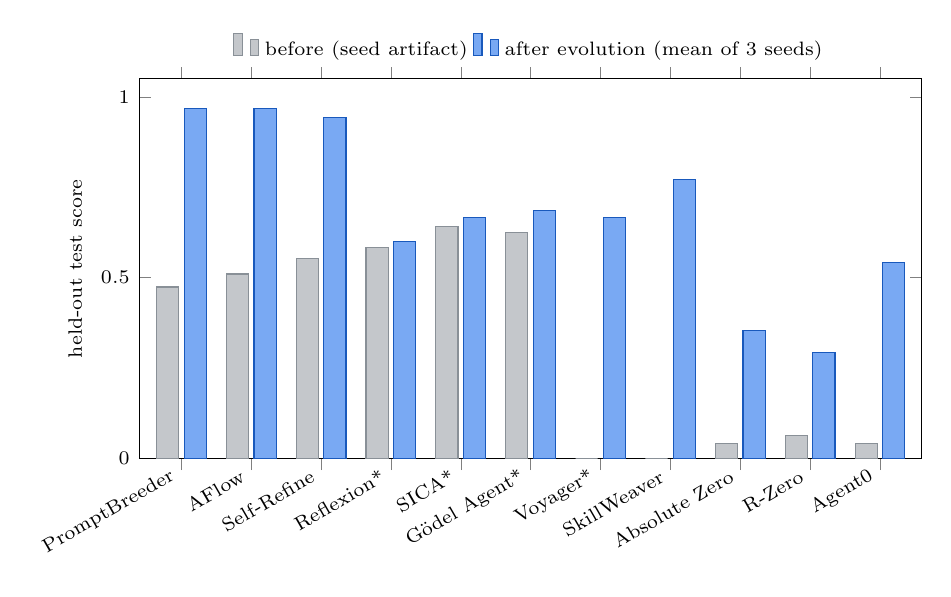
\begin{tikzpicture}
\begin{axis}[
  width=0.95\textwidth, height=6.4cm,
  ybar, bar width=8pt,
  ylabel={held-out test score},
  symbolic x coords={PromptBreeder, AFlow, Self-Refine, Reflexion*, SICA*, G\"odel Agent*, Voyager*, SkillWeaver, Absolute Zero, R-Zero, Agent0},
  xtick=data, x tick label style={rotate=30, anchor=east, font=\scriptsize},
  ymin=0, ymax=1.05, enlarge x limits=0.06,
  legend style={font=\scriptsize, at={(0.5,1.02)}, anchor=south, legend columns=2, draw=none, fill=none},
  tick label style={font=\scriptsize}, label style={font=\scriptsize},
]
\addplot[fill=adgray!35, draw=adgray!70] coordinates {
  (PromptBreeder,0.474) (AFlow,0.510) (Self-Refine,0.552) (Reflexion*,0.583)
  (SICA*,0.641) (G\"odel Agent*,0.625) (Voyager*,0.000) (SkillWeaver,0.000)
  (Absolute Zero,0.042) (R-Zero,0.062) (Agent0,0.042)};
\addlegendentry{before (seed artifact)}
\addplot[fill=adblue!60, draw=adblue!80!black] coordinates {
  (PromptBreeder,0.969) (AFlow,0.969) (Self-Refine,0.943) (Reflexion*,0.599)
  (SICA*,0.667) (G\"odel Agent*,0.687) (Voyager*,0.667) (SkillWeaver,0.771)
  (Absolute Zero,0.354) (R-Zero,0.292) (Agent0,0.542)};
\addlegendentry{after evolution (mean of 3 seeds)}
\end{axis}
\end{tikzpicture}
\caption{Held-out test score before and after evolution for the eleven microports and analogues, each run against \code{deepseek-v4-flash} under the \emph{most aggressive} configuration --- barrier-free async pipeline, 8 workers, Full staleness, 80 rollouts per seed, 3 seeds (465--2{,}069 model calls per seed). ``After'' bars are three-seed means; asterisked methods improved on two of three seeds (the rest on all three), and Reflexion's gain is within its domain's $\pm 0.02$ noise floor. Between 3 and 10 of the 240 proposals per method ($80 \times 3$ seeds) commit --- the gate admits only strict held-out improvements, so sparse acceptance is the shape of the mechanism, not a low yield. Bars are comparable only within a domain; per-seed spreads are tabulated in the repository documentation.}
\label{fig:eleven}
\end{figure}

Throughput is meaningful only if learning is preserved, so quality is measured under the most aggressive configuration (barrier-free, 8 workers, \textsc{Full} staleness). \Cref{fig:eleven} reports the eleven declarative ports at three seeds each. Read precisely, and more conservatively than an earlier draft did. Ten of eleven raise their three-seed mean test score, but a per-port paired $t$-test on three seeds ($t_{.975,2} = 4.303$) separates only six of them from zero: Reflexion, SICA, G\"odel Agent, R-Zero and Voyager do not, and four of those five are the methods that improved on two of three seeds rather than all three. The $\pm 0.02$ \emph{noise floor} an earlier draft applied uniformly is also not defensible across these splits, which range from 64 items to 8: on SkillWeaver's eight-task split one task is $0.125$, and Voyager's test metric takes only the values $0$ and $1$, so a $\pm 0.02$ floor is arithmetically impossible there. Bars are comparable only within a domain and the per-port $n$ differs by a factor of eight. Gains are bounded by each benchmark's headroom --- the three GSM8K ports converge to 0.94--0.97 and differ in cost rather than quality. What this establishes is that the most aggressive schedule the framework offers --- no barrier, eight workers, staleness admitted unconditionally --- does not stop published algorithms from learning on their own benchmarks; a paired serial-schedule arm at equal budget would additionally price asynchrony \emph{relative to serial}, and is left to future work. Among the benchmark-faithful ports, three representative single-seed results establish end-to-end operation (not effect sizes): ACE improves FiNER-139 \citep{loukas2022finer} validation $0.719 \to 0.766$ over 120 rollouts while curating a ten-bullet playbook; DGM's best archived child repairs held-out vendored bugs at $0.906$ versus its seed agent's $0.844$ under a frozen \code{pytest} oracle (a compact SWE-bench-style setting \citep{jimenez2023swebench}); SkillOpt improves a hard SearchQA \citep{dunn2017searchqa} subset $0.053 \to 0.211$ with 3 of 43 proposed edits accepted. One port produced no quality number at all: ADAS's benchmarks were either saturated (MGSM) or cost-prohibitive per call (GPQA), and we state this rather than average over it. The highest-level interface (\code{evolve\_skill}) on 40 HotpotQA rows raises held-out exact match from $0.167$ to $0.583$ over 338 model calls, committing one proposal.

\paragraph{Is the gate that decides this optimistic?} It reuses one fixed $\Dval$ across every decision, so an accepted diff is a selected extreme statistic on that split (\cref{sec:aggregator}). The 33 runs above measure the resulting bias directly, since each records both its $\Dval$ trajectory and its disjoint test score: mean val gain $+0.395$ against mean test gain $+0.357$, a mean gap of $-0.038$ (median $-0.031$, s.d.\ $0.075$), with test gain short of val gain in 20 of 33 runs and above it in 7 --- a two-sided sign test on the 27 non-tied runs gives $p = 0.019$. That test treats the 33 runs as independent, which they are not: they are 11 ports $\times$ 3 seeds, and seeds within a port share a benchmark, a $\Dval$, and a reward granularity. Taking the port as the unit gives 8 negative port means against 2 positive and 1 tied. A sign test on those 11 gives $p = 0.109$, but that test throws away every magnitude at the one sample size where they matter most; a paired $t$ on the port means gives $t = -2.49$ on 10 degrees of freedom, 95\% CI $[-0.073, -0.004]$, which excludes zero. The clustering objection is therefore answered without the effect disappearing: it survives at the port level when magnitude is used and not when it is discarded. The run-level result is also fragile: dropping any one of five of the eleven ports moves $p$ above $0.05$, and dropping SkillWeaver alone --- whose test split has eight items, so one task is $0.125$ --- moves the mean gap from $-0.038$ to $-0.026$. What we claim is therefore the direction and the magnitude, not significance: the optimism is consistently negative, about a tenth of the mean gain, concentrated in the coarsest-reward ports, and too small to change the sign of any result here, where every quality figure is reported on test.

\subsection{RQ4: Merge-of-$N$ versus best-of-$N$ selection at equal budget}
\label{sec:merge-vs-fork}
Throughput cannot distinguish merging from sampling-and-selecting, since $N$ independent forks occupy $N$ workers equally well; the discriminating quantity is held-out quality at an equal rollout budget. Two earlier attempts produced null results and are the reason \cref{eq:fusionrate} exists; both are plotted as the red markers of \cref{fig:fusionrate} and their configurations are in \cref{tab:config}. Neither measures a merging deficit --- in both, merging barely fired. On single-key HotpotQA the fused union was built twice in the whole experiment; on ACE's per-bullet playbook, where key granularity was supposed to be the fix, it fired no more often, because that artifact already scored $0.938$ on the gate's split, putting $f \approx 0.06$ and the predicted rate at $2\%$. The condition, not the granularity, was binding.

\Cref{eq:fusionrate} also prescribes the fix, so we built the workload it calls for. BBH \citep{suzgun2023bbh} supplies tasks a strong model still fails, and \code{KeyedRules} supplies an artifact keyed by the category a failure diagnosis falls into (output format, method, verification, common errors). Crossing them needed no engine change --- only a new \code{Workload}, because dataset and strategy are independent seams (\cref{sec:pluggable}). On \code{GLM-5.2} the seed artifact scores $0.100$ on test, so $f \approx 0.9$, and at $N{=}8$ \cref{eq:fusionrate} predicts that essentially every round should have something to fuse.

It does. Over a 32-rollout run the aggregator held \textbf{3 contested tournaments} --- the first in this project in which fusion actually ran --- while the artifact improved from $0.100$ to $0.400$ on test, so the workload supplies both the failure rate and the headroom the question needs. The fused candidate \textbf{won 1 of the 3}, at a mean gain of $-0.115$ with two losses (worst $-0.250$); two of the three fell below the artifact they started from. On this workload, fusing a round's diffs was usually \emph{worse} than keeping the better single one --- and the acceptance gate refused exactly those, which is the safeguard of \cref{sec:aggregator} behaving as designed rather than an argument against it.

With fusion firing on demand, the comparison the question has been waiting for becomes possible. We ran it at three seeds, and then --- because the three-seed reading was favorable to merging --- at three more. The second half did not replicate the first, and the combined result is the one we report: six seeds $\times$ three arms on \code{bbh-keyed}, 32 rollouts pinned on every arm, $N{=}8$, \code{GLM-5.2} (16{,}124 model calls, 28.3 hours of model time).

\begin{table}[t]
\centering
\footnotesize
\setlength{\tabcolsep}{5pt}
\caption{Merge-of-$N$ against best-of-$N$ selection and a serial control at an equal rollout budget, on a workload built to satisfy \cref{eq:fusionrate}, in two configurations. \emph{Test} is a split no gate in any arm ever saw; \emph{s.d.} is across seeds. \emph{Oracle} is the best fork \emph{on test}, an upper bound that requires the answer to select, against which the fork row reports what fork-and-select can actually ship. \emph{Calls} is the per-seed median. Wall-clock is deliberately not tabulated: the fork arm ran its $N$ sub-runs sequentially, so its recorded wall-clock is a sum rather than what $N$ concurrent forks would take, and the arms of a seed shared one endpoint. Model calls are unaffected by both and are the cost currency we report.}
\label{tab:mergefork}
\begin{tabular}{@{}llrrrrr@{}}
\toprule
& \textbf{arm} & \textbf{test min/med/max} & \textbf{mean} & \textbf{s.d.} & \textbf{oracle} & \textbf{calls} \\
\midrule
\multirow{3}{*}{\rotatebox{90}{\scriptsize $N{=}8$, 32}}
& serial     & 0.133 / \textbf{0.267} / 0.333 & \textbf{0.250} & 0.084 & ---   & 772  \\
& fork-of-8  & 0.067 / 0.200 / 0.300          & 0.189 & 0.093 & 0.267 & 1004 \\
& merge-of-8 & 0.033 / 0.217 / 0.400          & 0.194 & 0.142 & ---   & \textbf{685}  \\
\midrule
\multirow{3}{*}{\rotatebox{90}{\scriptsize $N{=}4$, 96}}
& serial     & 0.100 / 0.250 / 0.433          & 0.256 & 0.129 & ---   & 2070 \\
& fork-of-4  & 0.133 / \textbf{0.300} / 0.400 & \textbf{0.283} & 0.115 & 0.333 & 2363 \\
& merge-of-4 & 0.200 / 0.267 / 0.400          & 0.267 & \textbf{0.073} & ---   & \textbf{1832} \\
\bottomrule
\end{tabular}

\vspace{2pt}
{\scriptsize Both blocks: six seeds. Upper: 4 rounds per run. Lower: 24 rounds per run.}
\end{table}



\textbf{Merging is the cheapest arm at equal quality.} The framework's premise is throughput --- accepted improvement per unit wall-clock --- so the claim merging has to meet is non-inferiority in quality at lower cost. The six seeds deliver the cost half cleanly and the quality half only weakly. Quality: the paired merge${-}$fork difference is $+0.005$ with a 95\% interval of $[-0.186, +0.196]$ at $N{=}8$ and $-0.017$ with $[-0.133, +0.100]$ at $N{=}4$. Those intervals are wider than the arm means themselves ($0.19$--$0.28$), so what the design can detect is a penalty of roughly $0.16$--$0.26$ test-score points and nothing smaller. We report the intervals rather than a $p$-value because at six seeds with ties the sign test cannot reach $\alpha = 0.05$ at all --- its smallest attainable $p$ is $0.0625$ at $N{=}8$ and $0.125$ at $N{=}4$ --- so a non-significant result there carries no information. Cost, by contrast, is measured cleanly: merge is the cheapest arm in model calls --- $11\%$ fewer than serial and $22$--$32\%$ fewer than fork. Against fork this is the validation-cost mechanism of \cref{sec:lever-val} showing up as money: $N$ independent forks must each be scored where a round's survivors are scored once. Against \emph{serial} it cannot be, and we say so: a serial lineage produces one proposal per step, so $k = 1$ and collapsing $k$ tests into one predicts no saving at all. The $11\%$ we measure there must come from something else --- fewer proposals, because merge workers share what the others have already learned and more of their rollouts solve outright; or diffs discarded by the staleness filter before they reach the gate. Separating those needs a decomposition of calls into rollout, proposal and gate-evaluation counts, which the engine's counters permit and we have not reported.

\emph{We report no wall-clock advantage over fork, and an earlier draft's claim of one was wrong.} The fork arm's runs were executed sequentially (\code{-{}-fork-concurrency 1}), so the wall-clock we compared against was the \emph{sum} of $N$ forks rather than what $N$ concurrent forks would take. On the same runs the longest single fork is $320$--$376$\,s against merge's $1{,}127$--$1{,}176$\,s: given $N$ workers, fork-of-$N$ finishes a pinned rollout budget \emph{faster} than merge-of-$N$, because each fork is a short serial lineage with no round barrier and no shared gate. That is the honest comparison and it cuts against us on this axis. Merging's cost advantage is in model calls, where the gate is amortized; wall-clock at equal worker count belongs to selection.

Two bounds travel with the quality column. Seeds 0--2 alone put merge's median at $0.267$ against fork's $0.100$ and seeds 3--5 reversed it; we report the pooled six rather than the favorable half. The decision to run the second three was made \emph{after} seeing the first three and because they were favourable, which is data-dependent stopping: the six-seed figures are therefore descriptive, and we do not attach inferential weight to them beyond the intervals above. And six seeds on a 30-task split detect only large effects, so what is established is the absence of a large quality penalty.

\textbf{Fusion width is a design parameter, and \cref{eq:fusionrate} does not fix it alone.} The precondition is satisfied almost equally by $N{=}4$ ($99.6\%$ of rounds have something to fuse) and $N{=}8$ ($100\%$), but the two differ in what they do to the rest of the loop: at a fixed rollout budget $N{=}8$ halves the number of rounds, and therefore the opportunities to accumulate, while making each fused union an eight-way jump that the trust region of \cref{sec:aggregator} exists to prevent. Width should therefore be set at the smallest $N$ that clears \cref{eq:fusionrate}, not the largest available --- a concrete design rule the equation yields once the round count is priced in. Re-running at $N{=}4$ and a $3\times$ budget (24 rounds), also at six seeds, moves the mechanism in the predicted direction: the mean per-seed fusion gain rises from $-0.135$ to $-0.045$, and the merge arm's seed-to-seed standard deviation falls from $0.142$ --- the \emph{worst} of the three arms --- to $0.073$, the \emph{lowest}, against serial's $0.129$ and fork's $0.115$. None of these variance ratios is separable at six seeds (every $F$ is far inside the two-sided critical value at $5,5$ degrees of freedom), and the ordering reverses between the two widths, so we report it as an ordering with a mechanism attached and not as an effect. Quality remains indistinguishable within intervals as wide as those above, and merge remains the cheapest arm ($1832$ calls against $2070$ and $2363$).

That variance ordering is the observation we would most like to see tested properly, and six seeds cannot test it. It has a mechanism to its name --- merging averages several workers' evidence into one artifact, where selection keeps whichever single lineage the gate happened to prefer --- but the evidence has three problems we state rather than argue past: no variance ratio is significant at $n{=}6$, the ordering \emph{reverses} between the two widths, and the ratio halved when we went from three seeds to six. A quantity that flips across configurations and shrinks as the sample grows is what noise looks like. We record it as a hypothesis with a mechanism, not as a finding.

\textbf{The fusion counters, across both configurations.} At $N{=}8$ the aggregator held 10 contested tournaments over six seeds and the fused candidate won 2 ($20\%$); at $N{=}4$ it held 21 and won 4 ($19\%$), at a mean per-seed gain of $-0.045$ against width 8's $-0.135$. Fusion loses more contests than it wins in both --- and this is why the design works: the acceptance test refuses exactly those losses, so carrying a usually-worse union costs one gate sweep and nothing else, while the wins are kept. Non-inferior quality at a $20\%$ fusion win rate is the gate doing its job, not a result in spite of it. The negative control holds throughout: across eighteen control runs the serial and fork arms held 823 tournaments and contested \emph{none}, as their construction requires.

The summary is therefore narrower than an earlier draft of this paper claimed: \textbf{on this workload merging costs $11$--$32\%$ fewer model calls than the alternatives at a pinned rollout budget, and we cannot detect a quality difference at the resolution six seeds afford.} The cost result is the measured one; the quality result is an interval too wide to exclude penalties smaller than about $0.16$. Merging is not shown to improve quality, and it does not win on wall-clock.

\section{Limitations}
\label{sec:limits}

AgentDescent is a research reference implementation, and seven boundaries delimit what its evaluation establishes. (i) \emph{Effect sizes}. The quality results establish direction and rule out large penalties rather than measuring magnitudes: six seeds on a 30-task split in RQ4, four seeds for the reflective-merge ablation, three for the RQ1 ladder and the eleven-port study, one seed for each benchmark-faithful port. Merging is shown non-inferior and cheaper, not superior, and the variance ordering of \cref{sec:merge-vs-fork} is reported as a direction rather than a ratio. (ii) \emph{Scale}. The system is a single Python process --- one merger thread (measured at $75.7\%$ occupancy at $N{=}4$), thread workers, a local git ledger. Multi-machine operation, a contended CAS path, and a worker sweep beyond $N{=}8$ are outside this paper. We also cannot yet say \emph{what} the busy merger is busy with: the \code{merge\_seconds} and \code{merge\_gate\_seconds} timers wrap the same region in the released code, so the profile bounds the merger's occupancy but does not attribute it. Locating the saturation point needs both that decomposition and the sweep. (iii) \emph{Holdout reuse}. Measured in \cref{sec:exp-ports} and bounded there; no reusable-holdout or $\Dval$-rotation mechanism is implemented. (iv) \emph{Bounded staleness is designed, not measured}. \code{resync\_on\_commit} defaults to true in every run reported here, so the lag budget is never the only resynchronization trigger, and the runs record \code{stale\_considered} in the single digits or at zero. \Cref{eq:eta} and the \textsc{Guarded}/\textsc{Reflective} policies are therefore a design contribution in this paper and not an empirical one; an ablation with that flag off is the experiment that would change it. (v) \emph{Fault tolerance is implemented and unevaluated}. Worker retirement, merger backoff, the stall detector and the bounded shutdown are all in the engine; no experiment injects a fault, and the failures we do observe are endpoint errors we report as measured rather than as a recovery result. (vi) \emph{What withdrawing the scheduler matrix costs}. Asynchrony is now supported by RQ1 alone --- one port, one workload, three seeds --- and both the reflective-merge ablation and the merge-versus-selection comparison run synchronously. The claim that eighteen ports \emph{run} under all three schedulers rests on the ports' flag plumbing and on their barrier-free runs, not on a measured three-way comparison. A title foregrounding asynchrony is therefore ahead of its evidence, and the $N{=}8$ replacement sweep is the run that would settle it. (vii) \emph{Transfer}. A multi-algorithm scheduler matrix reported in an earlier draft is withdrawn from this one: it was measured at $N{=}2$ on the implementation preceding the ports' declarative restructuring, its raw per-run data was not retained, and at two workers the round barrier has almost nothing to hide, so it could not distinguish a property of the ports from a property of the width. Separately, difficulty parameters calibrated on one model did not transfer under a model swap, whereas benchmark-intrinsic difficulty did. Every number reported here is generated by a named script, and measurements that proved irreproducible or favorably defined --- including, in an earlier draft, a width-8 experiment withdrawn for a flawed control --- were re-measured and corrected in place. We regard that discipline as part of the contribution: the evaluation of a self-improving system should satisfy the standard its own acceptance gate imposes on diffs.

\section{Conclusion}
\label{sec:conclusion}

The distributed-training stack admits a coherent counterpart in agent self-evolution once its necessary disanalogy --- diffs do not add --- is taken seriously and merging is constructed as a discrete-space optimizer. Efficiency decomposes into three sources, and the third is the one specific to merging: rollout overlap and barrier removal take wall-clock from $790$ to $116$\,s against a faithful serial control, while reduced validation cost --- $k$ acceptance tests collapsed into one --- is the saving selection cannot have. That third source is where this paper spends its evidence, because it is the one with a precondition that can fail silently. Eighteen published algorithms adapt as plug-ins rather than forks --- eleven of them measured here, the rest ported but not used as evidence --- and all run under the three schedulers unmodified --- which is what makes the scheduler a controlled variable instead of a property of each paper's own loop. Merging has two preconditions and both can fail quietly. It needs two diffs to exist, which \cref{eq:fusionrate} states in closed form and which a near-saturated artifact violates however finely its keys are cut; and it needs them to be fusable, which a one-key artifact violates absolutely --- measured here as $0$ fused unions in $48$ merges. \emph{Reflective merge} is what removes the second failure, and isolating it gives the paper its clearest result: $42$ of $48$ merges fused, and $40\%$ fewer model calls than the shipped defaults at a pinned rollout budget (95\% CI $27$--$54\%$) --- traced, after we first misattributed it, to resolving contradictions by recombination rather than by ranking, since both configurations run exactly one acceptance test per merge. Quality is not the claim; four seeds on a 30-task split cannot support one, and we report the interval rather than assert equivalence. What the result does support is a way of accounting we would like to see adopted: a self-evolution loop should be judged on accepted improvement per unit of \emph{validation}, not per proposal, because validation is what it actually pays for.

\section*{Reproducibility}
\label{sec:repro}
\sloppy
All code is available at \url{https://github.com/Birfy/agentdescent} (MIT license; \code{pip install agentdescent}; the core engine has no required dependencies). Generating scripts, per result: thread overlap --- \code{examples/efficiency.py -{}-only gil}; RQ1 and the live merger profile of \cref{sec:lever-val} --- \code{bench/matrix\_run.py -{}-rows gepa}; RQ2 --- \code{bench/baselines\_run.py -{}-dataset bbh -{}-fetch 120}, run twice, once with \code{-{}-fusion-tournament} and once with \code{-{}-reflective-merge}; RQ3 --- each port's own command line over \code{examples/\_method\_runner.py}, the entry point that accepts the \code{-{}-staleness full} configuration used, with the resolved configuration printed as one JSON line per run; the \code{evolve\_skill} case --- \code{examples/skill\_evolution.py}; RQ4 --- \code{bench/baselines\_run.py -{}-dataset bbh-keyed -{}-fusion-tournament}, whose workload (BBH crossed with \code{KeyedRules}), width and budget sweeps, and fusion counters were added for this paper and ship with it. Every port supports \code{-{}-dry-run} (no API key or model call) and carries an offline test suite; datasets are retrieved from canonical sources by a dependency-free data layer.

\bibliographystyle{plainnat}
\bibliography{references}

\end{document}
